\section{Vítr jako morfogenetický činitel}
Vítr je ve srovnání s vodou výrazně slabším morfogenetickým a erozním činitelem. Nízká efektivita je způsobena především jeho nižší hustotou a viskozitou. Vítr tak dokáže zpravidla transportovat v suspenzi jen velmi malé částice. Stejně jako s rychlostí proudící vody roste její unášecí schopnost, roste s rychlostí i unášecí síla větru.

Vítr se morfogeneticky projevuje zejména v územích, kde chybí vegetační kryt a na povrchu je sypký, jemnozrnný materiál. Důležité je, aby povrch byl i suchý. Vlhkost totiž zvyšuje kohezi materiálu, jednotlivé částečky se k sobě lépe pojí. Vegetace taktéž zvyšuje soudržnost částeček a zároveň snižuje rychlost větru, což způsobuje vypadávání částic.
	
%\subsection{Charakteristiky větru a vlastnosti povrchu}
%
%
%Typy proudění vzduchu:
%
%\begin{itemize}
%	\item Laminární
%	\item Turbulentní
%	\item Spirálovitý
%\end{itemize}

\section{Eolická eroze}
Velikost částic, koheze a vegetační charakteristiky ovlivňují náchylnost povrchu k větrné erozi. Vlhkost, jílové částice, organický materiál přispívají k soudržnosti materiálu - tyto faktory chybí v oblasti horkých pouští, kde je tedy eolická eroze nejefektivnější.

\emph{Deflace} je proces odnosu uvolněných částic z povrchu v důsledku působení větru. Odvátím částeček vznikají deprese (sníženiny) nazývané jako \emph{deflační vana}. Jelikož vítr dokáže odnést jen určitou frakci, dochází k \emph{selektivní deflaci}. Dochází tak k pasivní akumulaci větších klastů a vzniku tzv. \emph{pouštní dlažby}.

\emph{Koraze (abraze)} je geomorfologické působení částic obsažených ve vzduchovém proudu.

\section{Transport sedimentů}
Transport sedimentů vzduchem je podobný tomu ve vodě. Rozlišujeme čtyři základní typy transportu (Obr. \ref{fig:eoltransport}): v \emph{suspenzi}, \emph{saltací}, \emph{vlečením (ploužením)} a vymršťováním zrníček těmi dopadajícími (anglicky označované \emph{\enquote{reptation}}) \parencite{livingstoneAeolianGeomorphologyNew2019}. 

\begin{figure}
	\centering
	\includegraphics[width=1\linewidth]{obrazky/eolicka/eol_transport}
	\caption{Čtyři typy eolického transportu (upraveno podle \textcite{livingstoneAeolianGeomorphologyNew2019})}
	\label{fig:eoltransport}
\end{figure}


Nejjemnější sedimenty jsou transportovány v \emph{suspenzi} (\enquote{suspension}). Vítr dokáže donést nejjemnější částečky až na stovky a tisíce kilometrů daleko (Obr \ref{fig:zdrojprachu}). Není vůbec neobvyklé, že se do střední Evropy dostává prach ze Sahary. Díky dálkovému transportu prachu ze Sahary se do Amazonského deštného pralesa dostává velké množství živin, zejména fosforu \parencite{prosperoCharacterizingQuantifyingAfrican2020}.

\begin{figure*}
	\centering
	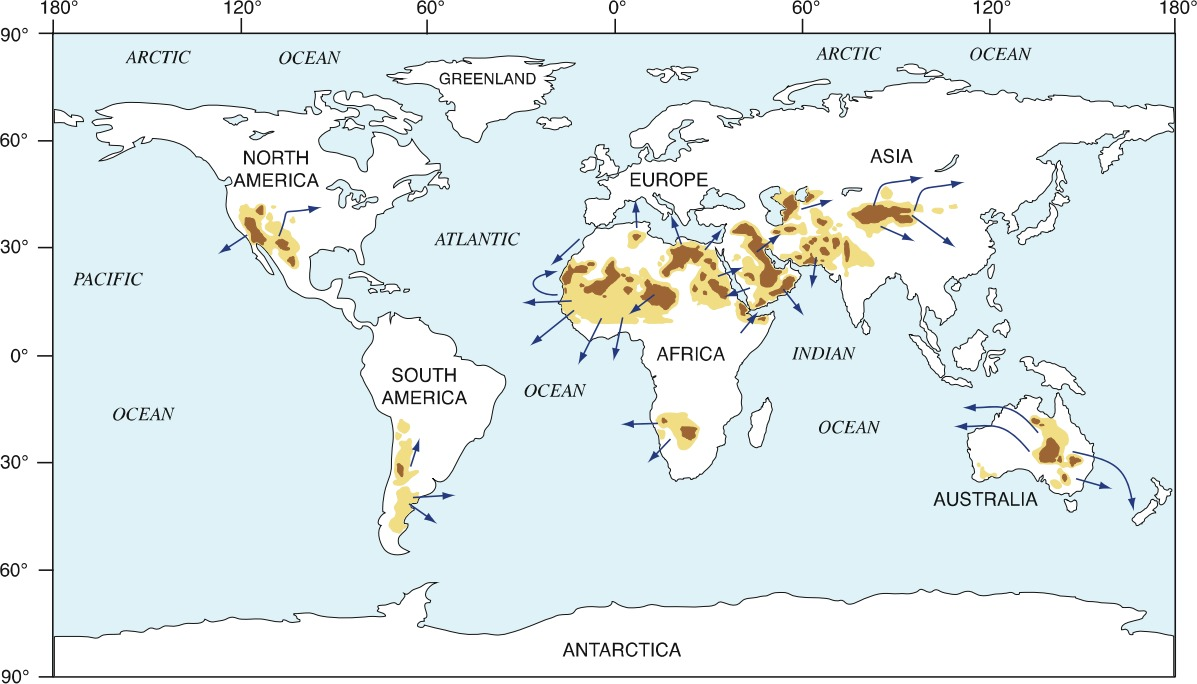
\includegraphics[width=1\linewidth]{obrazky/eolicka/zdroje_prachu}
	\caption{Světové zdrojové oblasti prachu a směry jeho transportu (zdroj: \textcite{muhsIdentifyingSourcesAeolian2014})}
	\label{fig:zdrojprachu}
\end{figure*}

Hrubší částečky se přesouvají \emph{saltací} (\enquote{saltation}). Jedná se o proces, kdy je klast větrem vyzdvižen a po chvilce letu vzduchem dopadá zpět na zem. V podstatě to je poskakování jednotlivých zrníček. Většina zrn je vyzdvižena maximálně do cca \SI{10}{\milli\metre} nad povrch a přenesena do vzdálenosti \SIrange{0,5}{1,5}{\metre}.

Klasty, které jsou natoli těžké, že je vítr nedokáže zvednout se po povrchu sunou nebo kutálí. Souhrnně se tento pohyb označuje jako \emph{ploužení} (\enquote{creep}).

Poslední, čtvrtý typ označovaný anglicky \emph{\enquote{reptation}}. Dopadající zrnka, která se pohybují saltací dokážou vymrštit ty klidně ležící. Pohyb vymrštěných zrnek je jen na velice krátkou vzdálenost (cca v řádech milimetrů).

\begin{figure*}
	\centering
	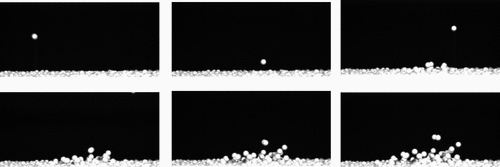
\includegraphics[width=1\linewidth]{obrazky/eolicka/saltace_foto}
	\caption{Sekvence fotografií pořízených během čtyř milisekund. Horní řádek: zrnko pohybující se saltací dopadá na povrch a odskakuje. Spodní řádek: Vymrštění částeček -- \enquote{reptation}. (Převzato z \textcite{beladjineCollisionProcessIncident2007})}
	\label{fig:saltacefoto}
\end{figure*}


%\section{Depozice sedimentů}
%
%Když unášecí schopnost větru poklesne (např. snížením jeho rychlosti), tedy sedimentační rychlos
%\todo[inline]{dopsat}

\section{Erozní formy}
Obrušováním větších klastů (valounky, balvany) nebo drobných výchozů podloží částečkami unášenými větrem vznikají \emph{hrance} (Obr. \ref{fig:hranec}). Hrance se vyznačují jednou nebo více vybroušenými ploškami \emph{facetami}. Jedna dominantní faceta odpovídá převládajícímu směru větru. Pokud má hranec více facet, je to spíše způsobené pohybem klastu než změnou směru větru \parencite{livingstoneAeolianGeomorphologyNew2019}.
\begin{figure}
	\centering
	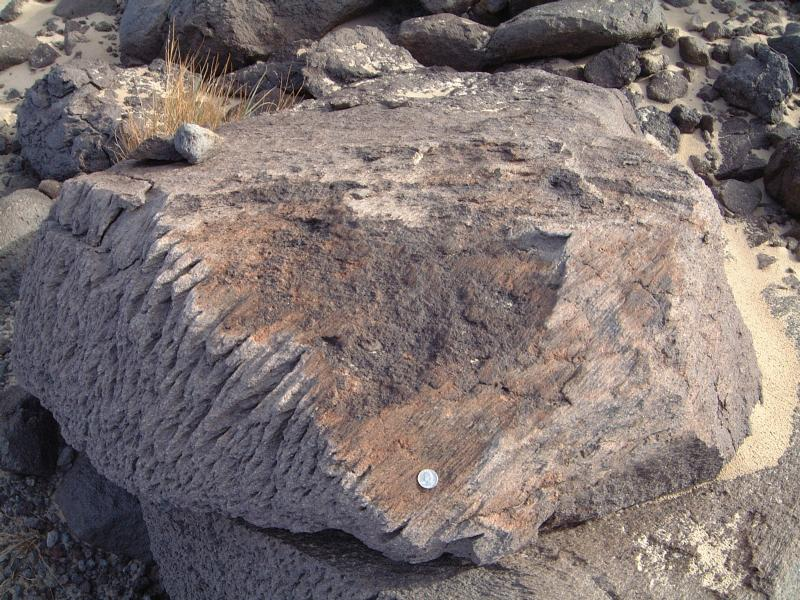
\includegraphics[width=1\linewidth]{obrazky/eolicka/ventifact_mojave}
	\caption{Hranec v Mohavské poušti (zdroj: Wikimedia Commons, volné dílo)}
	\label{fig:hranec}
\end{figure}

\emph{Jardangy} (\textit{yardangs}) jsou nízké, protáhlé hřbety, které mají směr totožný se směrem převládajícího větru. Vznikají v suchých oblastech se silnými větry jednoho převládající směru a s podložím tvořeným málo odolnými sedimentárními horninami. Jardangy se nacházejí zpravidla na velkých plochách, kde je několik těchto paralelních hřbítků. Jardangy vznikají korazí -- obrušováním větrem nesených částeček a deflací uvolněného materiálu. 

\emph{Hamada} je rozsáhlá kamenitá plocha (kamenité pouště). Jedná se o planiny pokryté ostrohrannými klasty velikosti valounů až balvanů. Jemný materiál zcela chybí, neboť podlehnul deflaci. \emph{Pouštní dlažba} je podobná hamadě. Zásadní rozdíl je v podobě klastů. Pouštní dlažba je tvořena menšími, suboválnými klasty, které jsou navíc do sebe zaklesnuté. Tvoří tak armorovaný povrch, který chrání podloží z nekonsolidovaných sedimentů před další erozí. 

\emph{Deflační pánve (vany)} (\enquote{deflation basin}) jsou mělké deprese které vznikly odnosem jemnozrného materiálu. Jedna z největších deflačních pánví -- Qattara Depressiuon v Egyptě má na délku okolo \SI{300}{\kilo\metre}, šířku \SI{145}{\kilo\metre} a dosahuje hloubky $134$ metrů pod mořem \parencite{albrittonOriginQattaraDepression1990}. V mnoha případech je dno pánve v úrovni hladiny podzemní vody a vznikají tam oázy. 

Vítr erozně působí jen do omezené výšky. Díky tomu mohou vznikat i tzv. \emph{skalní hřiby}.

\section{Akumulační formy}
Nejmenší eolickým akumulačním tvarem jsou \emph{čeřiny}. Jedná se o drobné hřbítky, které jsou kolmo na směr větru. Vznikají na površích tvořených sypkým materiálem. Nemají dlouhou životnost. 

\subsection{Písečné duny}
Zřejmě nejznámějším eolickým tvarem jsou \emph{písečné duny} (přesypy). Jedná se o elevace tvořené navátým pískem. Duny vznikají díky poklesu rychlosti větru pod transportní rychlost. Pokles rychlosti je zpravidla zapříčiněn přítomností nějaké překážky (skalní výchoz, vegetace...). 

Základní dělení dun je na tzv. \emph{volné duny} a \emph{vázané duny}. Volné duny jsou formovan0 pouze činností větru, který volně přemisťuje písek. Podle tvaru se volné duny dále rozdělují na příčné, lineární a hvězdicové. 

\begin{figure*}
	\centering
	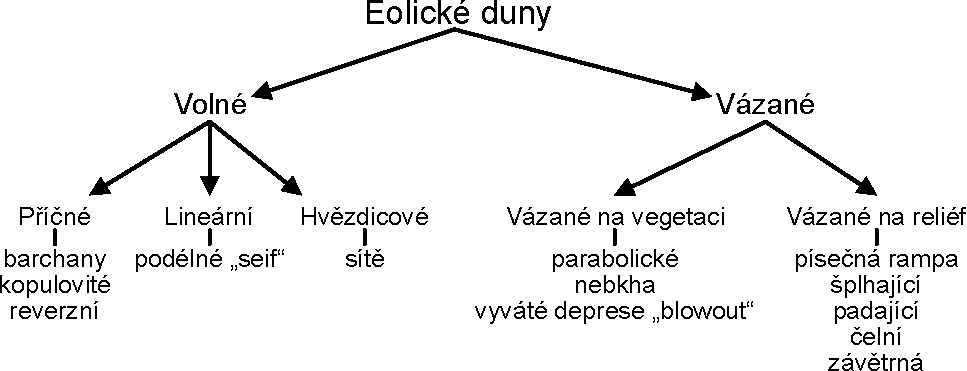
\includegraphics[width=1\linewidth]{obrazky/eolicka/typy_dun}
	\caption{Klasifikace dun (upraveno podle \textcite{livingstoneAeolianGeomorphologyNew2019})}
	\label{fig:typdun}
\end{figure*}

\subsection{Volné duny}
Tvar volných dun je výsledkem mnoha faktorů. Zjednodušeně lze říct, že tvar duny závisí na množství písku v území a variabilitě směru větru (Obr. \ref{fig:volneduny}). 

\emph{Barchany} neboli také \emph{srpovité duny} vznikají v oblastech, kde je málo písku a převládá jeden směr větru. Střední část barchanu je kolmo na směr proudění větru. Směrem k okrajům se ohýbá po směru větru a špičky jsou cca paralelní se směrem proudění. Duny na pobřeží mají čast tvar barchanů. Návětrná strana má sklon v rozmezí \SIrange{10}{14}{\degree}. Sklon závětrné strany je blízko sypnému úhlu suchého písku (okolo \SIrange{32}{34}{\degree}). S nárůstem množství materiálu se barchany propojují a vznikají \emph{příčné duny}. Jelikož se tyto duny nacházejí v oblastech kde dominuje vítr z jednoho směru, jedná se o nejmobilnější duny. Rychlost migrace dun je závislá na celkové hmotě duny. Menší duny migrují rychleji, neboť stačí transportovat méně hmoty, než u velkých dun. Barchany a příčné duny tvoří asi $10 \%$ všech dun \parencite{breedMorphologyDistributionDunes1979}.

Pokud je území vystaveno dvěma převládajícím směrům větru (polovinu roku fouká jedním směrem, polovinu  druhým) a písčitého materiálu podobně jako v oblasti batrchanů, vytvářejí se \emph{podélné duny} (\textit{linear dunes} nebo také \textit{longitudinal dunes}, Obr. \ref{fig:linearniduny}). Jedná se o nejběžnější typ písečných dun. Mají podobu klikatících se (sinusoidních) hřbetů. Dosahují výšky až \SI{200}{\metre} a na délku mohou mít i stovky kilometrů. Podélné duny jsou poměrně stabilní, což může vyhovovat vegetaci, která se uchycuje ve spodních partiích dun.

\begin{figure*}
	\centering
	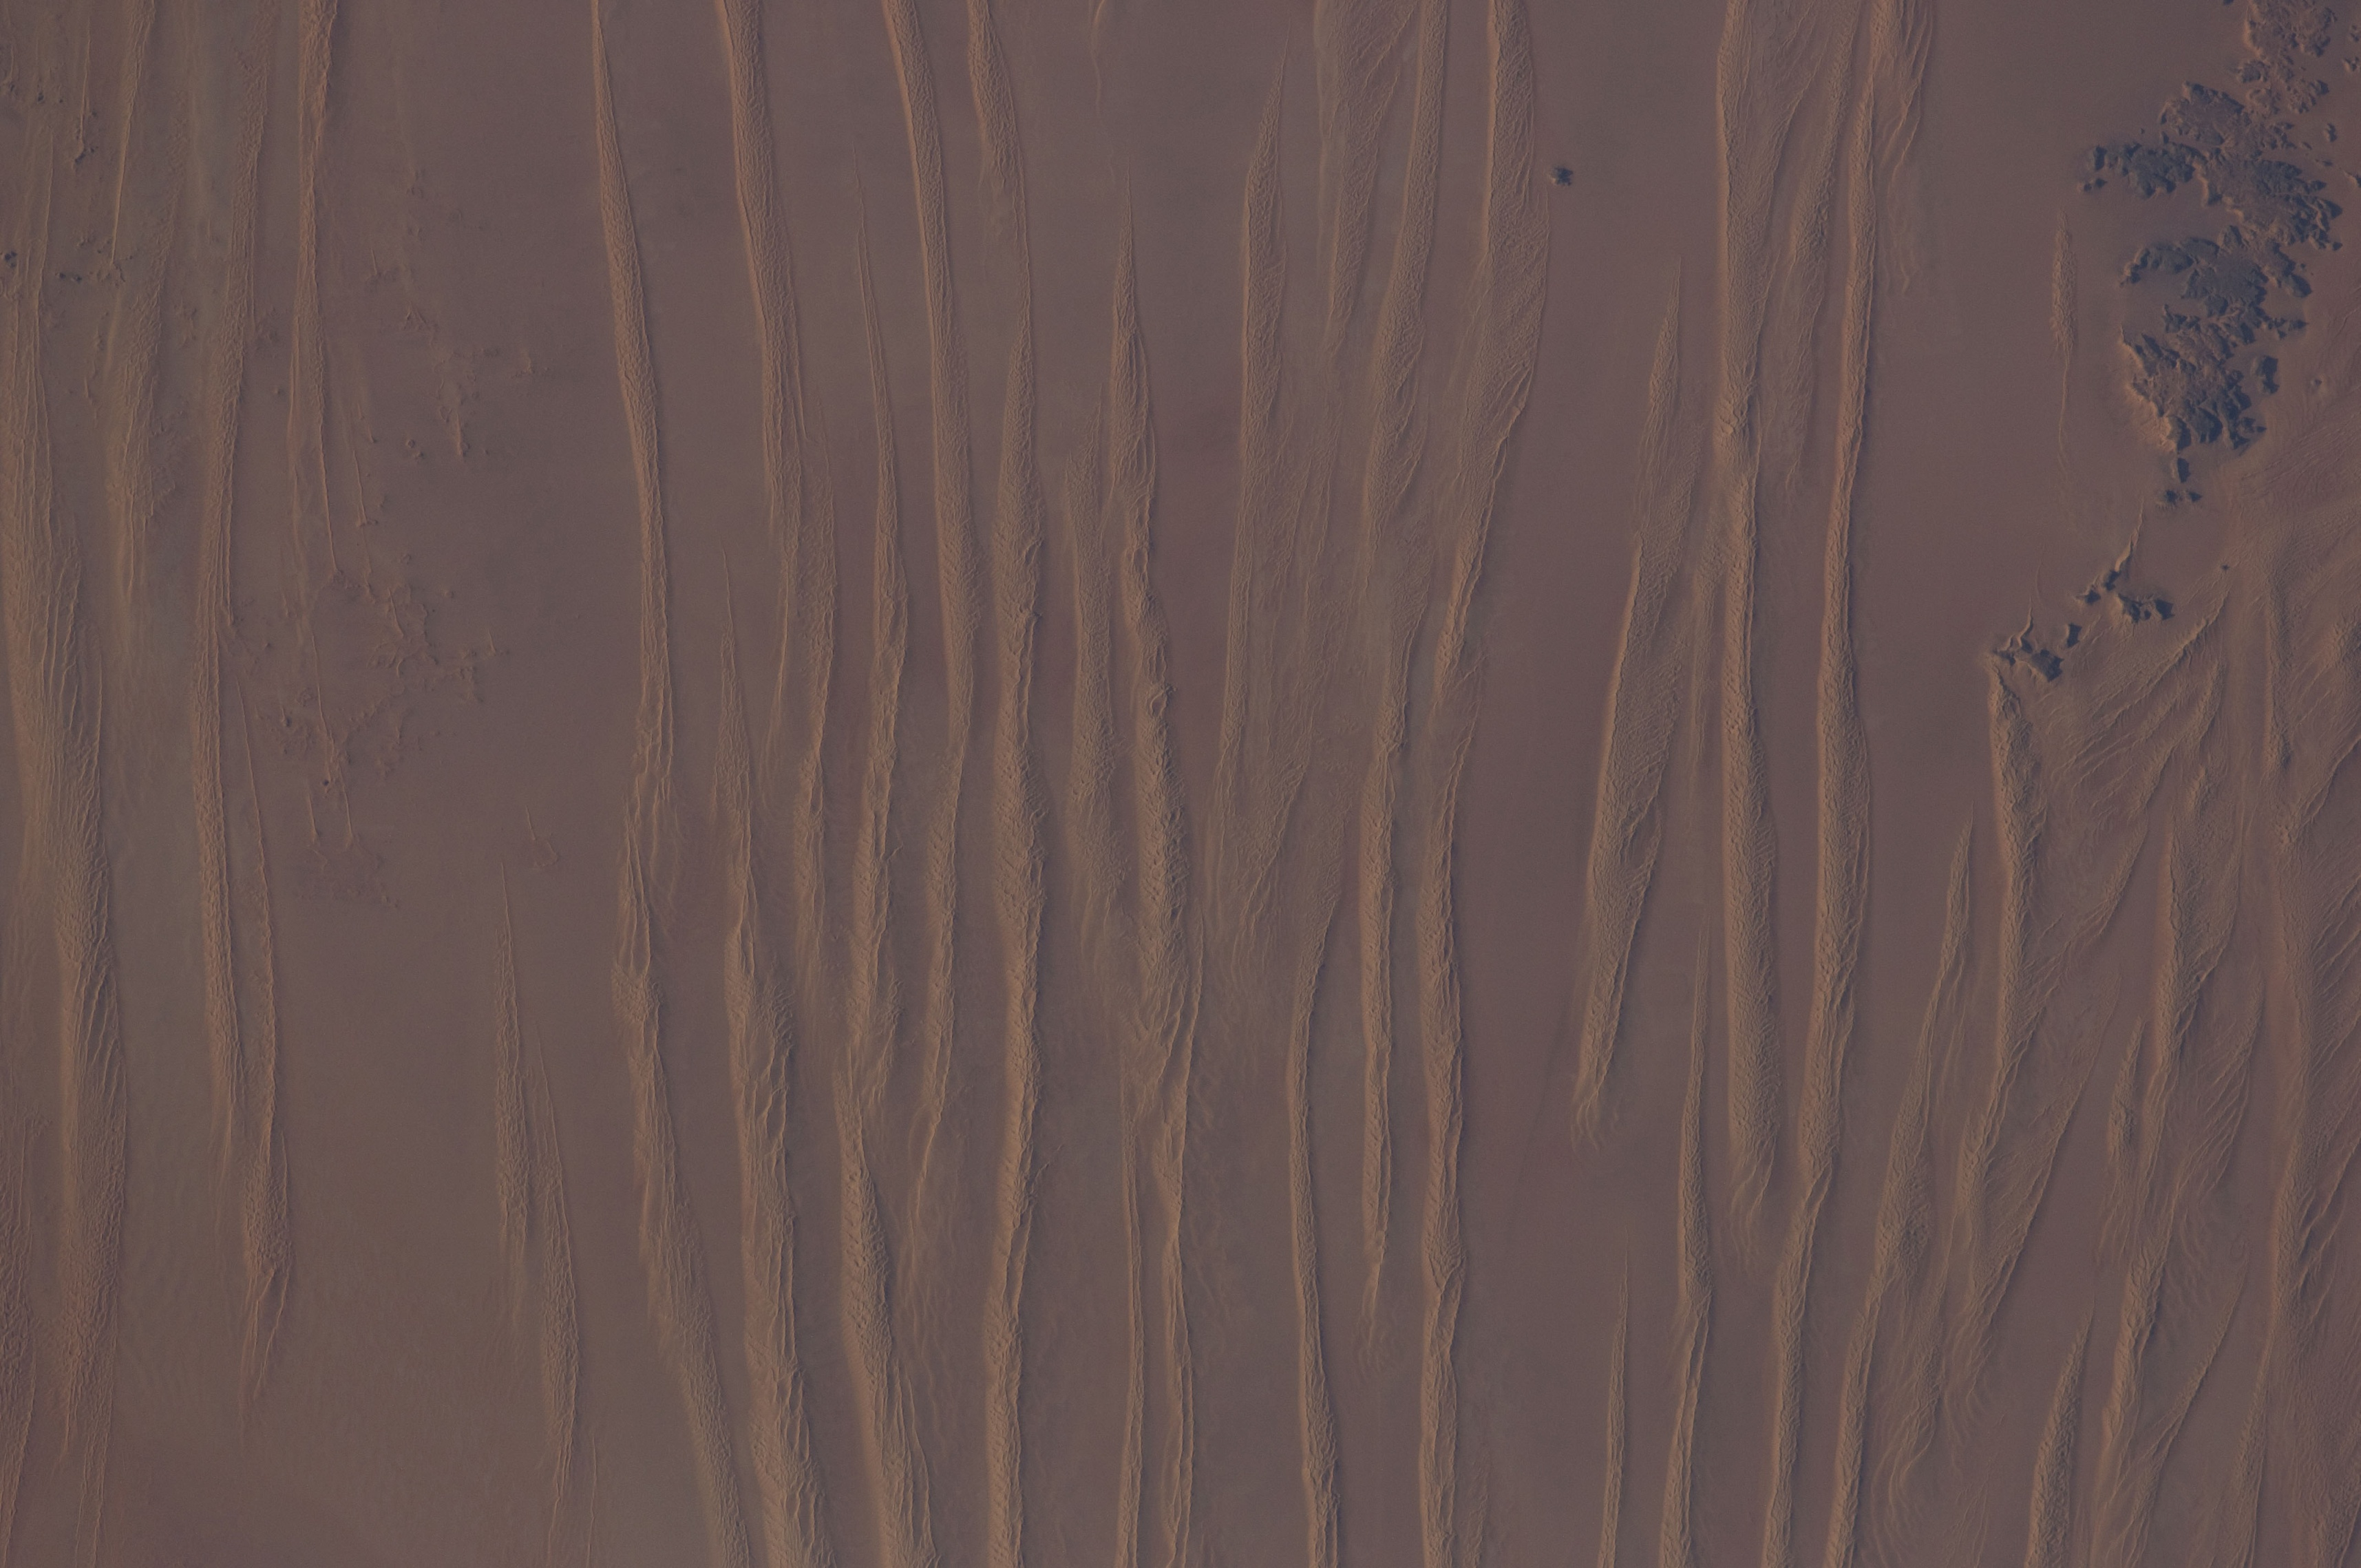
\includegraphics[width=1\linewidth]{obrazky/eolicka/linearniduny}
	\caption{Lineární duny ve Velkém písečném moři v jihozápadním Egyptě. Vzdálenost mezi dunama se pohybuje od \SIrange{1,5}{2,5}{\kilo\metre} (Fotografie pořízená z ISS, zdroj: NASA)}
	\label{fig:linearniduny}
\end{figure*}


\emph{Hvězdicové duny} jsou v oblastech s velkou variabilitou větru. Jedná se o rozsáhlá tělesa o výšce až \SI{300}{\metre}. Duna se skládá z menších \enquote{ramen}, které jednotlivým směrům větru.

\begin{figure}
	\centering
	\includegraphics[width=1\linewidth]{obrazky/eolicka/volne_duny}
	\caption{Závislost typu volných dun na mocnosti písku (při rovnoměrném rozložení v ploše) a variabilitě směru větru(upraveno podle \textcite{wassonFactorsDeterminingDesert1983})}
	\label{fig:volneduny}
\end{figure}

\subsection{Vázané duny}
Jako \emph{vázané duny} označujeme takové, které jsou přikotvené k nějaké překážce růyného tvaru a velikosti.

\emph{Nebkha} je duna, která vázaná na vegetaci zachytávající zrnka prachu, písku, ale i větších klastů. Velikost nebkhy může být od centimetrů (v iniciálních stádiích) až po více jak \SI{10}{\metre}. Podoba vegetace, na kterou jsou nebkhy vázané, silně ovlivňuje jejich morfologii.

\emph{Vyváté deprese} (\textit{blowouts}) jsou prohlubně rozličných tvarů. Nachází se v oblastech pokrytých sporadickou vegetací.

\emph{Parabolické duny} mohou vznikat po větru od vyvátých depresí. V půdorysu připomínají písmeno \enquote*{U} nebo \enquote*{V}. Narozdíl od barchanů jsou jejich výběžky otočené proti směru větru.

\emph{Lunety} jsou duny vznikají na okrajích jezer, playas. Jsou tvořeny zejména jílovou frakcí s variabilní příměsí písčité frakce. Jedná se o sedimenty vyváté ze dna bývalých jezer.

\emph{Čelní duny} jsou částo pobřežní duny vázané na pionýrská vegetaci. Označují se tak ale i duny před malou topografickou překážkou. Duny vzniklé až za překážkou jsou závětrné duny (\textit{lee dunes}).

Před velkou topografickou bariérou (např. skalní stěna, hřbety),  mohou vzniknout duny typu \emph{echo}, které věrně kopírují průběh překážky. Duny nasedající na bariéru z návětrné strany nazýváme \emph{šplhající duny} (\textit{climbing dunes}). Jejich méně strmá varianta je označována jako \emph{písečná rampa} (\textit{sand ramp}). Na závětrné straně překážky se vyskytují \emph{padající duny}.

\section{Spraš}
Spraš (\textit{loess}) je eolický sediment tvořený hlavně siltem (prach, frakce \SIrange{0,01}{0,05}{\milli\metre}) s významnou příměsí \ce{CaCO3}. Má okrovou barvu, což je způsobené přítomností oxidů železa. Spraše pokrývají 5--10 \% zemského povrchu (Obr. \ref{fig:spras_distribuce}) \textcite{biermanKeyConceptsGeomorphology2014}. Převážná část spraší se nachází na severní polokouli ve středních zeměpisných šířkách. Mocnost sprašových akumulací se pohybuje od centimetrů až po stovky metrů. 

Materiál spraší má rozličný původ. Významným zdrojem prachu byly v glaciálech rozsáhlé předledovcové plošiny, kde tavné vody z ledovců ukládaly velké množství materiálu. V jiných oblastech jsou zdrojem půdy vzniklé na málo odolných horninách (prachovce), případně rozsáhlé nížiny se sporým porostem vegetace. V současné době jsou zdrojem prachu hlavně pouštní oblasti.

Spraš je významným kvartérním sedimentem nejen střední Evropy. Díky zachování mocných akumulací jsou významným archivem uchovávajícím velké množství informací o kvartéru. Rychlost ukládání spraší se v průběhu kvartéru měnila. Během glaciálu se ukládalo největší množství, neboť podnebí bylo větrnější, sušší, chladnější. Při interglaciálech byla rychlost sedimentace snížena. Navíc vlhčí podmínky a větší množství vegetace umožnily rychlejší pedogenezi -- vznik půd. Během dalšího glaciálu byly tyto půdy pohřbené pod další vrstvou spraše. Opakováním těchto glaciálních a interglaciálních cyklů (případně i kratších výkyvů) vznikaly sekvence pohřbených půd. 

\begin{landscape}
	\begin{figure}
		\centering
		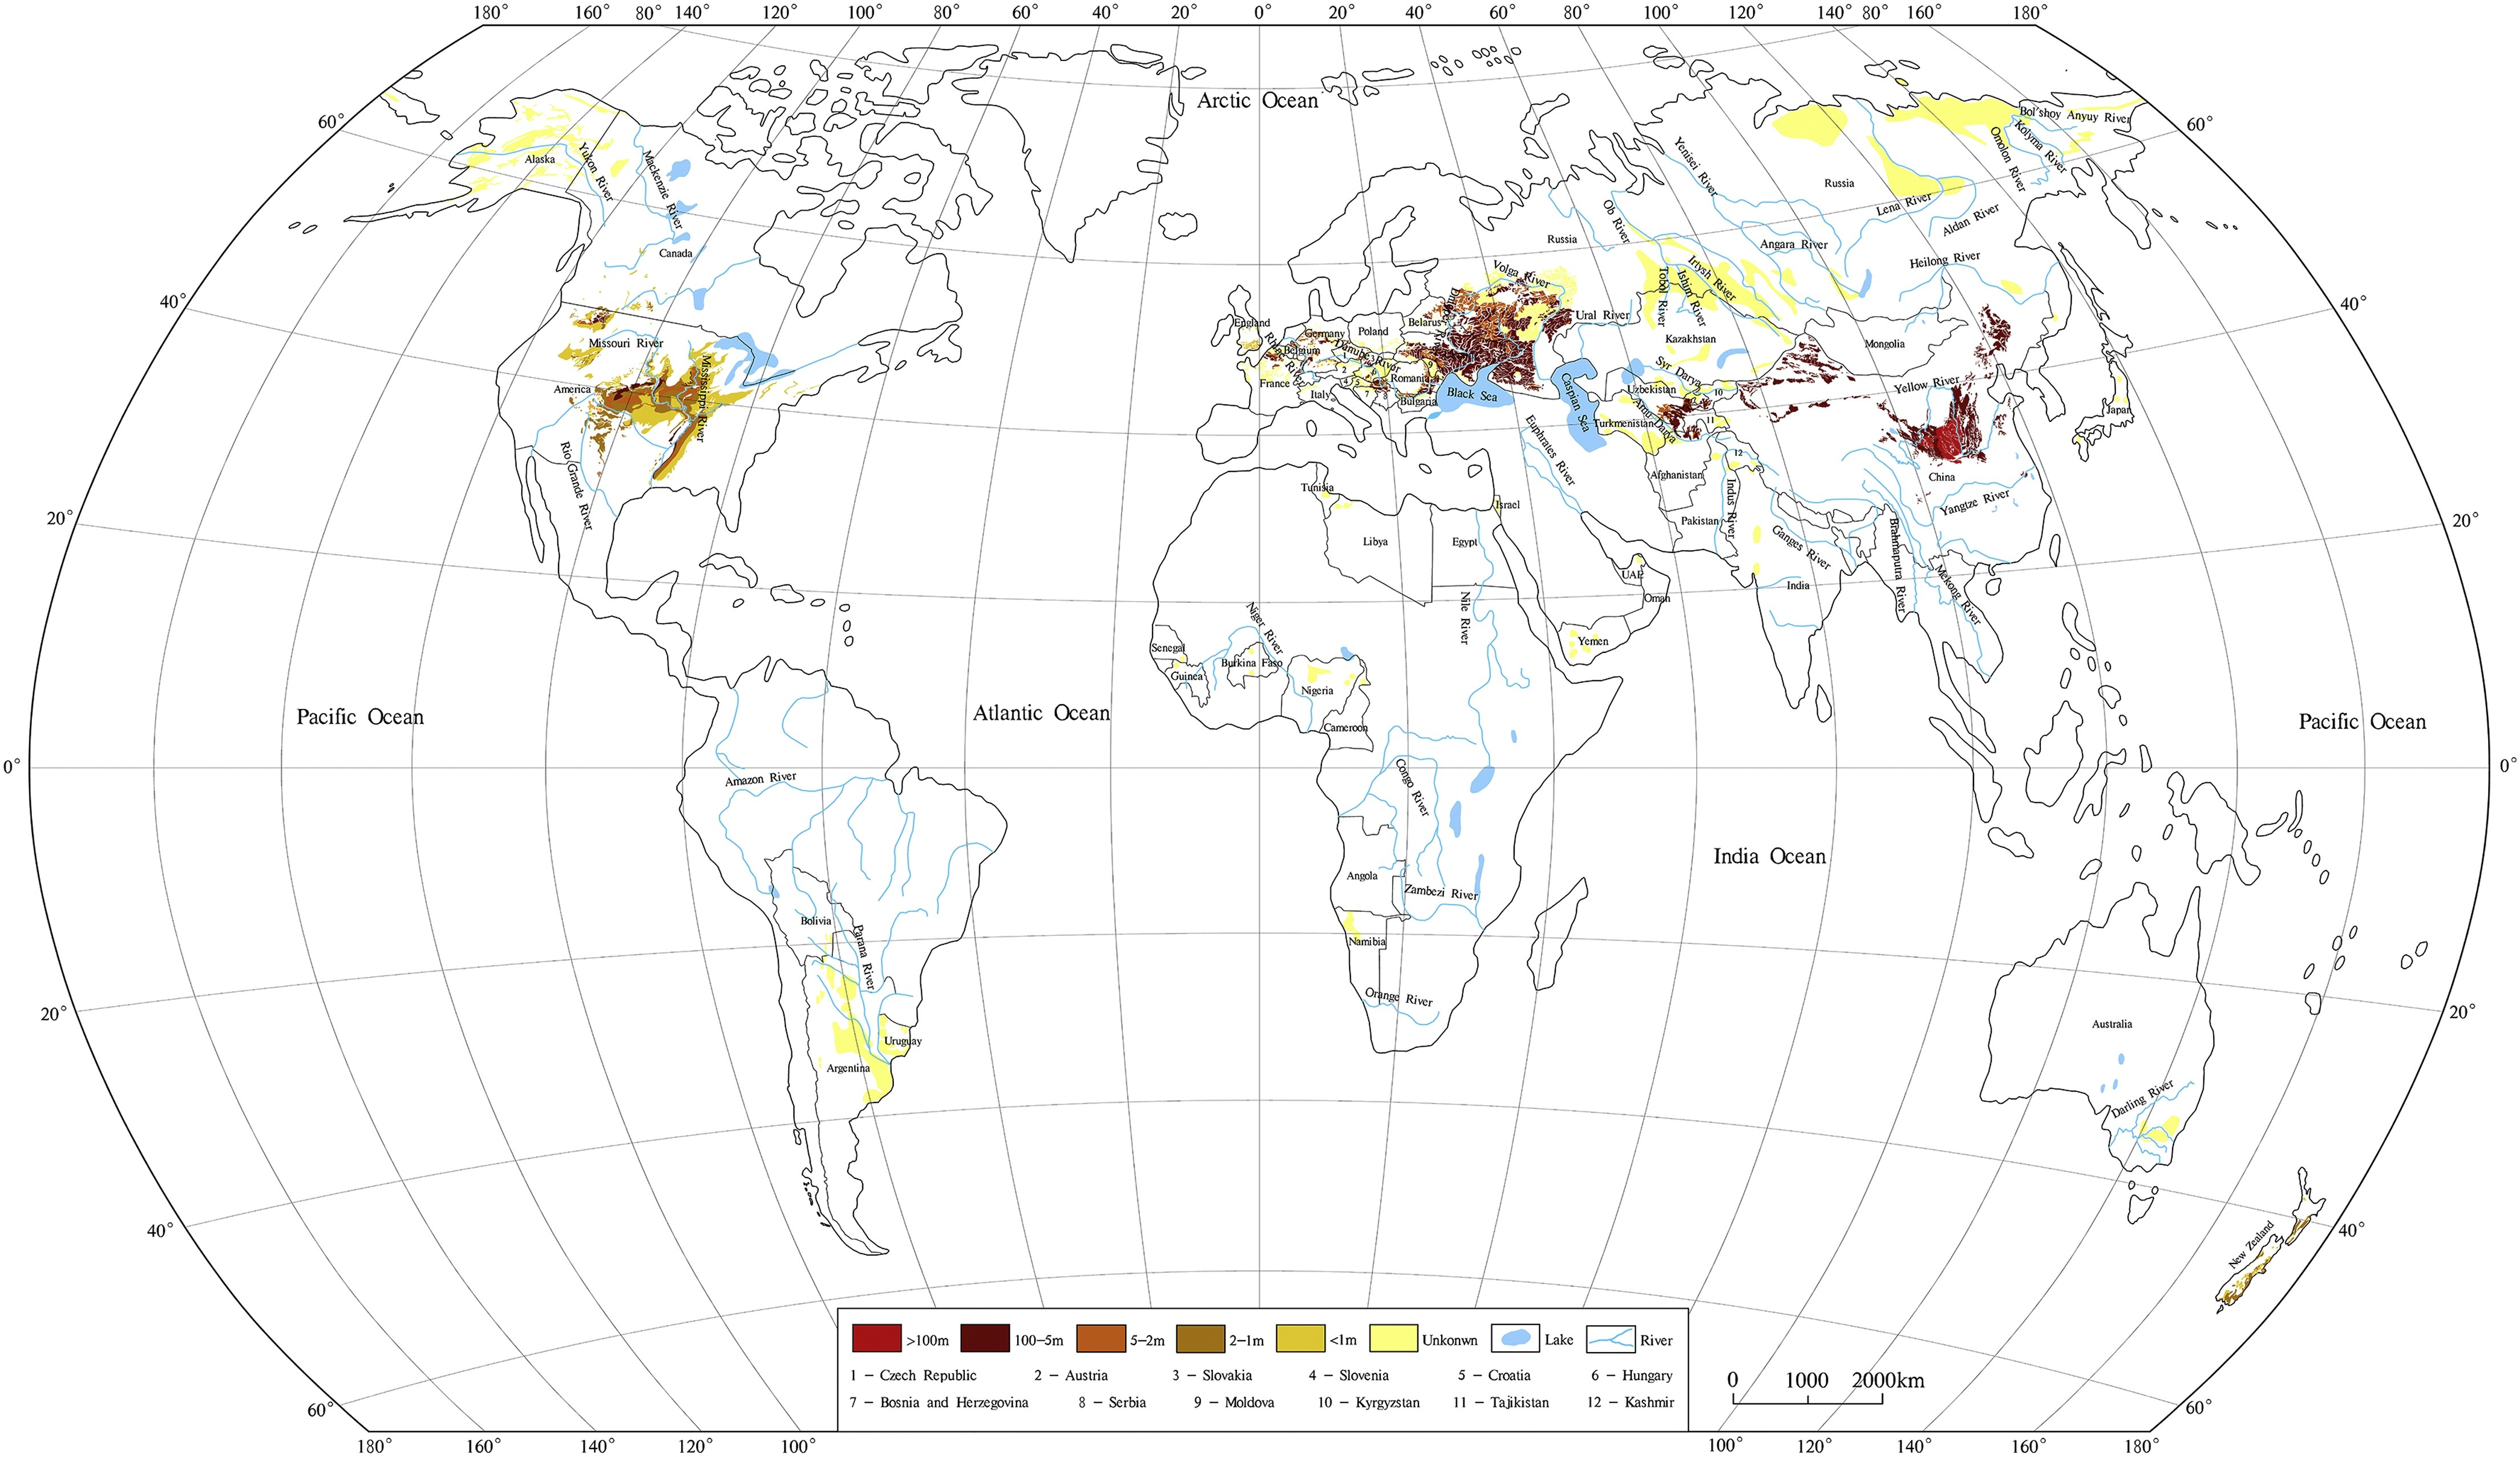
\includegraphics[width=1\linewidth]{obrazky/eolicka/loes_distr}
		\caption{Rozšíření spraše a její mocnost (zdroj: \textcite{liLoessGenesisWorldwide2020}}
		\label{fig:spras_distribuce}
	\end{figure}
\end{landscape}


\newpage
\onecolumn
\begin{boxotazky}{Kontrolní a klíčové otázky, na které bychom měli znát odpověď}
	\begin{itemize}
		\item 
		\item 
		
	\end{itemize}
\end{boxotazky}

\begin{boxslovnik}{Další klíčové pojmy k zapamatování}
	aaa & adfasd \\
	
\end{boxslovnik}
\twocolumn